\begin{chapter}{Testing and Validation}
  \begin{section}{Tests}
    During the development of the library some tests were developed in order to test behavior in the changing code. They can be run with \(\texttt{cargo test}\). Tests don't cover all code branches, but have been written for pieces of code that might break more easily. Tests are usually present in a separate file as the structure declaration and have the suffix ``\_test.rs'' in their name, so that they might be easily recognized.

    For example in the workspace \(\texttt{bisimilarity}\) tests have been written for the algorithms implemented.

\begin{minted}{Rust}
#[test]
fn bisimilar_paige_tarjan_3() {
  use petgraph::Graph;
  let mut graph_b = Graph::new();

  let node_b_1 = graph_b.add_node(1);
  let node_b_2 = graph_b.add_node(2);
  graph_b.add_edge(node_b_1, node_b_2, 1);
  let node_b_3 = graph_b.add_node(3);
  graph_b.add_edge(node_b_2, node_b_3, 2);
  let node_b_4 = graph_b.add_node(4);
  graph_b.add_edge(node_b_3, node_b_4, 2);

  let mut graph_c = Graph::new();

  let node_c_1 = graph_c.add_node(1);
  let node_c_2 = graph_c.add_node(2);
  graph_c.add_edge(node_c_1, node_c_2, 1);
  let node_c_3 = graph_c.add_node(3);
  graph_c.add_edge(node_c_2, node_c_3, 2);
  let node_c_4 = graph_c.add_node(4);
  graph_c.add_edge(node_c_3, node_c_4, 2);
  let node_c_5 = graph_c.add_node(5);
  graph_c.add_edge(node_c_1, node_c_5, 1);
  graph_c.add_edge(node_c_5, node_c_3, 2);

  assert!(bisimilarity(&&graph_b, &&graph_c));
  assert!(bisimilarity_ignore_labels(&&graph_b, &&graph_c))
}
\end{minted}

    The macro call \(\texttt{\#[test]}\) instructs rust to treat the function as a test and thus generate the respective code only when building for the test suite. Then the two graphs are constructed; finally the results are tested with the \(\texttt{assert!}\) macro.

    The structure of the two graph can be seen in figure\ \ref{graph_paige_tarjan_3}.

    \begin{minipage}{\textwidth}
      \centering
      \begin{minipage}[b][][b]{0.25\textwidth}
        \centering
        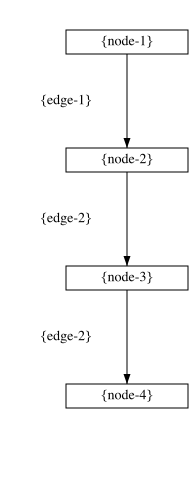
\includegraphics[width=\textwidth, angle=0]{figures/straight.pdf}
      \end{minipage}%
      \begin{minipage}[b][][b]{0.49\textwidth}
        \centering
        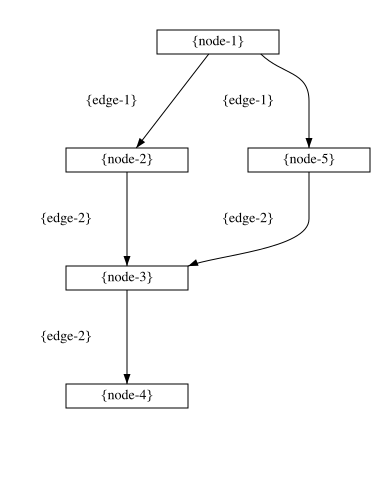
\includegraphics[width=\textwidth, angle=0]{figures/bifurcated.pdf}
      \end{minipage}%
      \captionsetup{type=figure}
      \caption{Graphs of tests}\label{graph_paige_tarjan_3}
    \end{minipage}\vspace{1em}

    The behavior of the two systems is the same by ignoring the labels on the edges and by considering them, so they are always bisimilar, so the test should not panic.

    The graphs have been generated using ReactionSystemsGUI using the nodes displayed in figure\ \ref{generating_graphs}. Note that to differentiate the two edges exiting \(\texttt{node-1}\) additional entities \(\texttt{left}\) and \(\texttt{right}\) are used, but are not displayed because the function for displaying the edges masks only for \(\texttt{edge-1}\) and \(\texttt{edge-2}\).

    \begin{minipage}{\textwidth}
      \centering
      \begin{minipage}{0.8\textwidth}
        \centering
        \includegraphics[width=\textwidth]{figures/straight_gui.png}
      \end{minipage}%

      \begin{minipage}{0.8\textwidth}
        \centering
        \includegraphics[width=\textwidth]{figures/bifurcated_gui.png}
      \end{minipage}%
      \captionsetup{type=figure}
      \caption{Generating graphs using ReactionSystemsGUI}\label{generating_graphs}
    \end{minipage}\vspace{1em}

    In addition to automated tests, some example inputs are provided in the folder \href{https://github.com/elvisrossi/ReactionSystems/tree/master/testing}{{\tt testing}}. The extension \(\texttt{.system}\) symbolizes system and associated instructions; the extension \(\texttt{.experiment}\) symbolizes an experiment, see\ \ref{experiment}.

    These examples were also used to do manual integration testing.

    The example \(\texttt{target.system}\)
    \begin{figure}[!ht]
      \centering
\begin{minted}{Text}
Environment: [x = {a}.y, y =({a}.{a, b}.nill + {b}.nill) ]
Initial Entities: {a, b}
Context: [({a,b}.{a}.{a,c}.x + {a,b}.{a}.{a}.nill)]
Reactions: ([{a,b}, {c}, {b}])

Target > Print,
Target (Limit: 7) > Print,
Target (Limit: 6) > Print,
Target (Limit: 5) > Print
\end{minted}
      \phantomsubcaption\label{example_target_system_instructions}
    \end{figure}
    generates as output:

\begin{minted}{Text}
After 6 steps we arrive at state:
{b}
After 6 steps we arrive at state:
{b}
After 6 steps we arrive at state:
{b}
After 5 steps we arrive at state:
{}
\end{minted}

    The output is correct since, as we can see from the graph of the system in figure\ \ref{graph_target_system} that the system has as leftmost production six states and the end state has entities set \(\texttt{\{b\}}\).

    \begin{figure}[h]
      \centering
      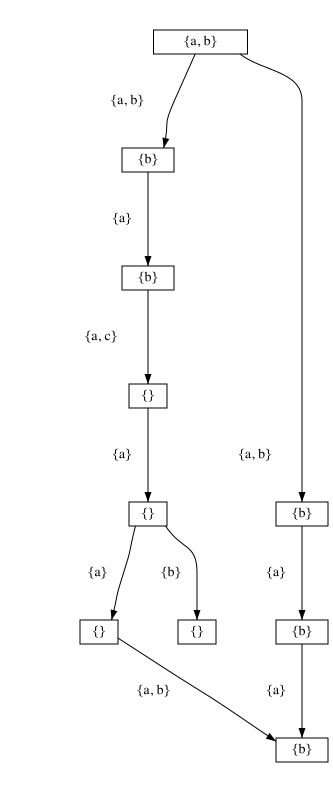
\includegraphics[width=0.5\textwidth, height=0.46\textheight, keepaspectratio]{figures/target_system.pdf}
      \caption{Graph of example\ \ref{example_target_system_instructions}, nodes have available entities as label, edges have the entities provided by the context as labels.}\label{graph_target_system}
    \end{figure}

    A small Perl script is provided that can convert systems created for the Prolog version of the program into the syntax described in\ \ref{design_system}. The script was used to convert systems that model mutual exclusion (MEX) available in the folder \href{https://github.com/elvisrossi/ReactionSystems/tree/master/testing/mex}{\(\texttt{testing/mex}\)}.

    A MEX system is composed of \(n\) looping processes, which only one can be in the critical section. Each process is identified by \(\texttt{out\_i}\) if is out of the critical section, \(\texttt{req\_i}\) if has requested to enter the critical section and \(\texttt{in\_i}\) if is in the critical section. Without the token \(\texttt{act\_i}\) no process can change state:

\begin{minted}{Text}
[{out_1}, {act_1}, {out_1}];
[{req_1}, {act_1}, {req_1}];
[{in_1}, {act_1}, {in_1}];
\end{minted}

    And \(\texttt{act\_i}\) is required to change state:

\begin{minted}{Text}
[{out_1, act_1}, {}, {req_1}];
\end{minted}

    Any subset of processes can be activated, the requests are preserved:

\begin{minted}{Text}
[{req_1, act_1, act_2}, {}, {req_1}];
[{req_1, act_1, act_3}, {}, {req_1}];
...
[{req_1, act_1, act_n}, {}, {req_1}];
\end{minted}

    Entering the critical section is handled by two other entities: \(\texttt{lock}\), which symbolizes that a process is in the critical section, and \(\texttt{done}\), which symbolizes that the critical section has been exited. \(\texttt{lock}\) remains until done:

\begin{minted}{Text}
[{lock}, {done}, {lock}];
\end{minted}

    No other processes have to have the lock for a process to enter the critical section:

\begin{minted}{Text}
[{req_1,act_1},{lock,act_2,...,act_n},{in_1,lock}];
\end{minted}

    The execution of these examples is more computationally expensive with increasing \(n\). The execution of \(\texttt{mex10.system}\) took 78791.202 milliseconds to run the instruction\ \ref{instruction_mex} which generate the graph of the system, converts it to dot format and saves it.\vspace{1em}

    \begin{minipage}{\textwidth}
\begin{minted}{Text}
Digraph > Dot
	| Entities
	| Context
	| ! "white"
	| ! "black"
	> Save("out.dot")
\end{minted}
      \captionsetup{type=table, name=\textbf{Instruction}}
      \caption{Instruction for MEX systems.}\label{instruction_mex}
    \end{minipage}\vspace{1em}

    \(\texttt{mex5.system}\) takes instead 109.148 milliseconds to run.

    Performance has been analyzed using perf\cite{manualperf_2025} and flamegraph\cite{Ochtman2025}.

    \begin{figure}
      \centering
      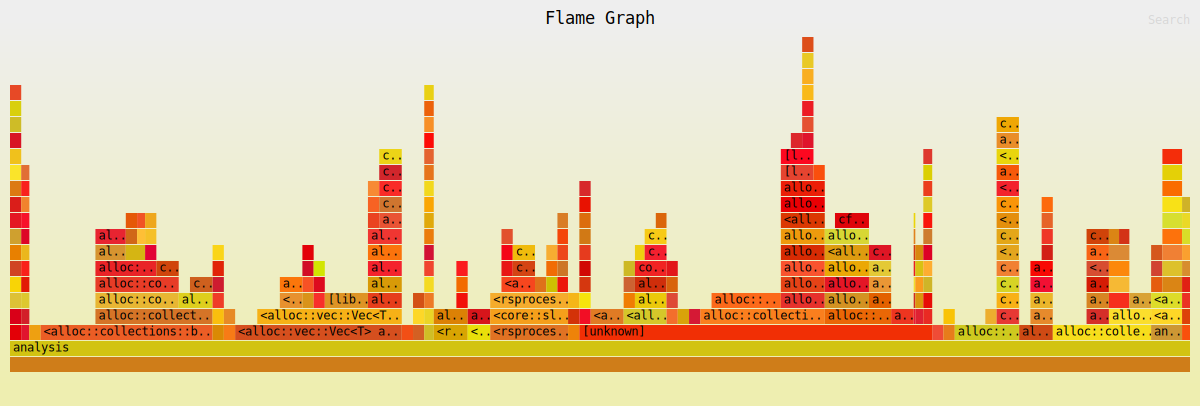
\includegraphics[width=\textwidth, height=0.5\textheight, keepaspectratio]{figures/flamegraph_mex5.pdf}
      \caption{Flamegraph of MEX RS with 5 processes.}
    \end{figure}

    \begin{figure}
      \centering
      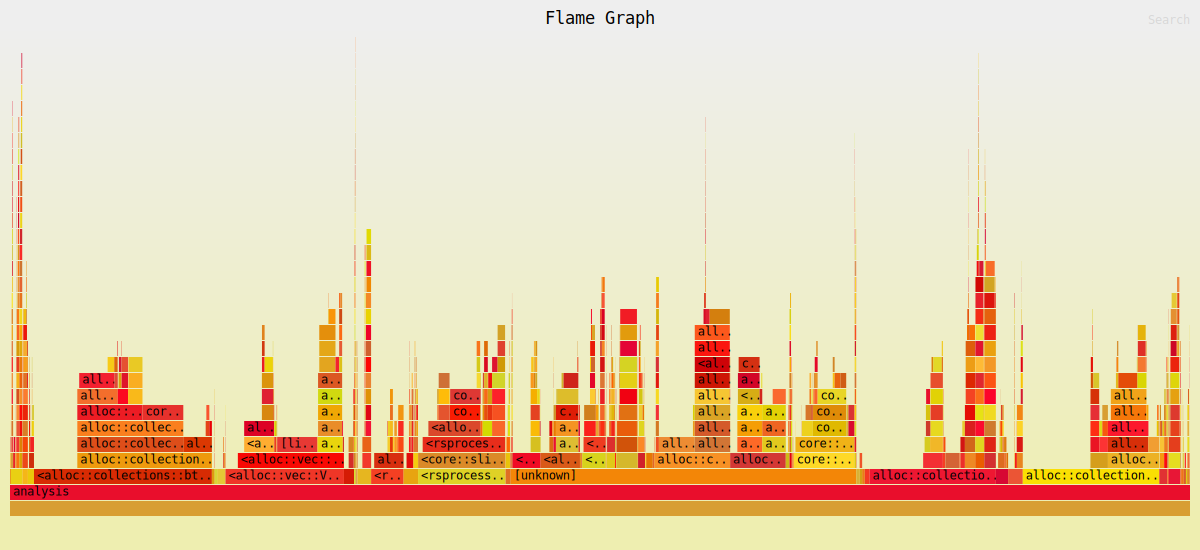
\includegraphics[width=\textwidth, height=0.5\textheight, keepaspectratio]{figures/flamegraph_mex10.pdf}
      \caption{Flamegraph of MEX RS with 10 processes.}
    \end{figure}

    Both of the flamegraphs share distinct features, but the one regarding MEX RS with 10 processes has finer resolution since the execution time is much longer. In decreasing order, some of the  that took most samples are:

    \begin{itemize}
    \item \(\texttt{unknown}\) that took 29\% of samples,
    \item \(\texttt{alloc::collections::btree::map::IntoIter::dying\_next}\) that took 14\% of samples,
    \item \(\texttt{<alloc::collections::btree::map::Iter as}\\\texttt{ core::iter::traits::iterator::Iterator>::next}\) that took 11\% of samples,
    \item \(\texttt{alloc::collections::btree::append::::bulk\_push}\) that took 11\% of samples,
    \item \(\texttt{alloc::collections::btree::map::BTreeMap::bulk\_build\_from\_sorted\_iter}\) that took 5,1\% of samples,
    \item \(\ldots\)
    \end{itemize}

    From the perf data we can gather that parsing took less than 3\% of total time, and that \(\texttt{unknown}\) refers to the methods belonging to System (section\ \ref{development_system}). This behavior is expected since most of the computation is carried by the structure that generates the graph.
  \end{section}

  \begin{section}{Validation}
    During development key issues identified from previous projects where performance and usability. The biggest problem with Prolog software is exceeding the stack limit and thus running out of memory. This problem is completely solved by using Rust. Another problem was that of performance. On dot file generation a 2 to 7 times performance improvement is seen, depending on the model simulated.

    Usability has been taken into account both for an end user and for a programmer that intend to expand the system: grammar follows general rules largely compatible with previous projects; the grammar is decoupled from the internal representation and thus permits greater maintainability and expandability; the use of traits permits more modularity and the coexistence of multiple types of RS in the same project; domain specific languages allow more efficient and intuitive instruction specification; the graphical user interface presents instructions and methods over reaction systems in a more intuitive way that with just a command line interface; the node system allows greater modularity and for easy additions of new instructions; easy SVG generation reduce the time spent between different software and speeds up the end user's tasks; saving the state of the application allows for lower friction when switching between projects; the web GUI provides a platform agnostic interface for quick development.
    Thus the original goal to develop a more user-friendly and developer-friendly reaction system modeler has been met.
  \end{section}
\end{chapter}
